% Chapter 2

\chapter{Computación en Nube para Móviles} % Main chapter title

\label{Chapter3} % For referencing the chapter elsewhere, use \ref{Chapter1} 

\lhead{Capítulo 3. \emph{Computación en nube para móviles}} % This is for the header on each page - perhaps a shortened title

%----------------------------------------------------------------------------------------

El área de la computación en nube para móviles al ser un campo de investigación relativamente nuevo, no existe una definición
ampliamente aceptada y puede ser vista desde muchos ángulos como lo realizó el trabajo de  Fernando, Loke y Rahayu 
\cite{fernando2013mobile}, tomando hasta 3 definiciones distintas. En este trabajo nos referimos a MCC como un conjunto de técnicas que 
aprovechan los potentes recursos computacionales en nube para potenciar aplicaciones móviles con el principal objetivo de mejorar la calidad de 
servicio hacia los usuarios que tienen dispositivos limitados en términos de energía, procesamiento y almacenamiento. En este capítulo
detallaremos la visión actual de MCC, del mismo modo explicaremos la heterogeneidad que la envuelve,
y los desafíos por solucionar en las técnicas de \textit{offloading}.

\section{Visión}

MCC permite a los usuarios móviles acceder a sus aplicaciones, datos, y servicios en nube a través de internet aprovechando 
la web móvil \cite{dinh2013survey}, consiguiendo no depender totalmente de los recursos locales de los móviles,
, por tanto esta nueva ola tecnológica puede ser aplicada en varias áreas como la salud, negocios de TI, educación,
entretenimiento y redes sociales. 

En el trabajo de Abolfazli, Sanaei y Gani \cite{abolfazli2012mobile} se clasifica los enfoques
que puede tomar la mejora en los dispositivos móviles entre hardware y software los cuales se muestran en la gráfica de la Figura
\ref{fig:approachesmobileaugmentation}.  Si bien los avances de hardware son virtuosos, son aún lentos en comparación a la creciente 
expectativa de los usuarios y desarrolladores de aplicaciones. Otro enfoque alternativo para la mejora de las capacidades computacionales 
de los dispositivos es usar técnicas de software 
para la conservación de recursos
locales y la reducción de requerimientos de recursos al instalar aplicaciones. En consecuencia, sostenemos que la computación en nube 
tendrá una participación
destacada aventajándose de valiosos recursos remotos con el fin de mejorar la experiencia del usuario.

\begin{figure}[h]
 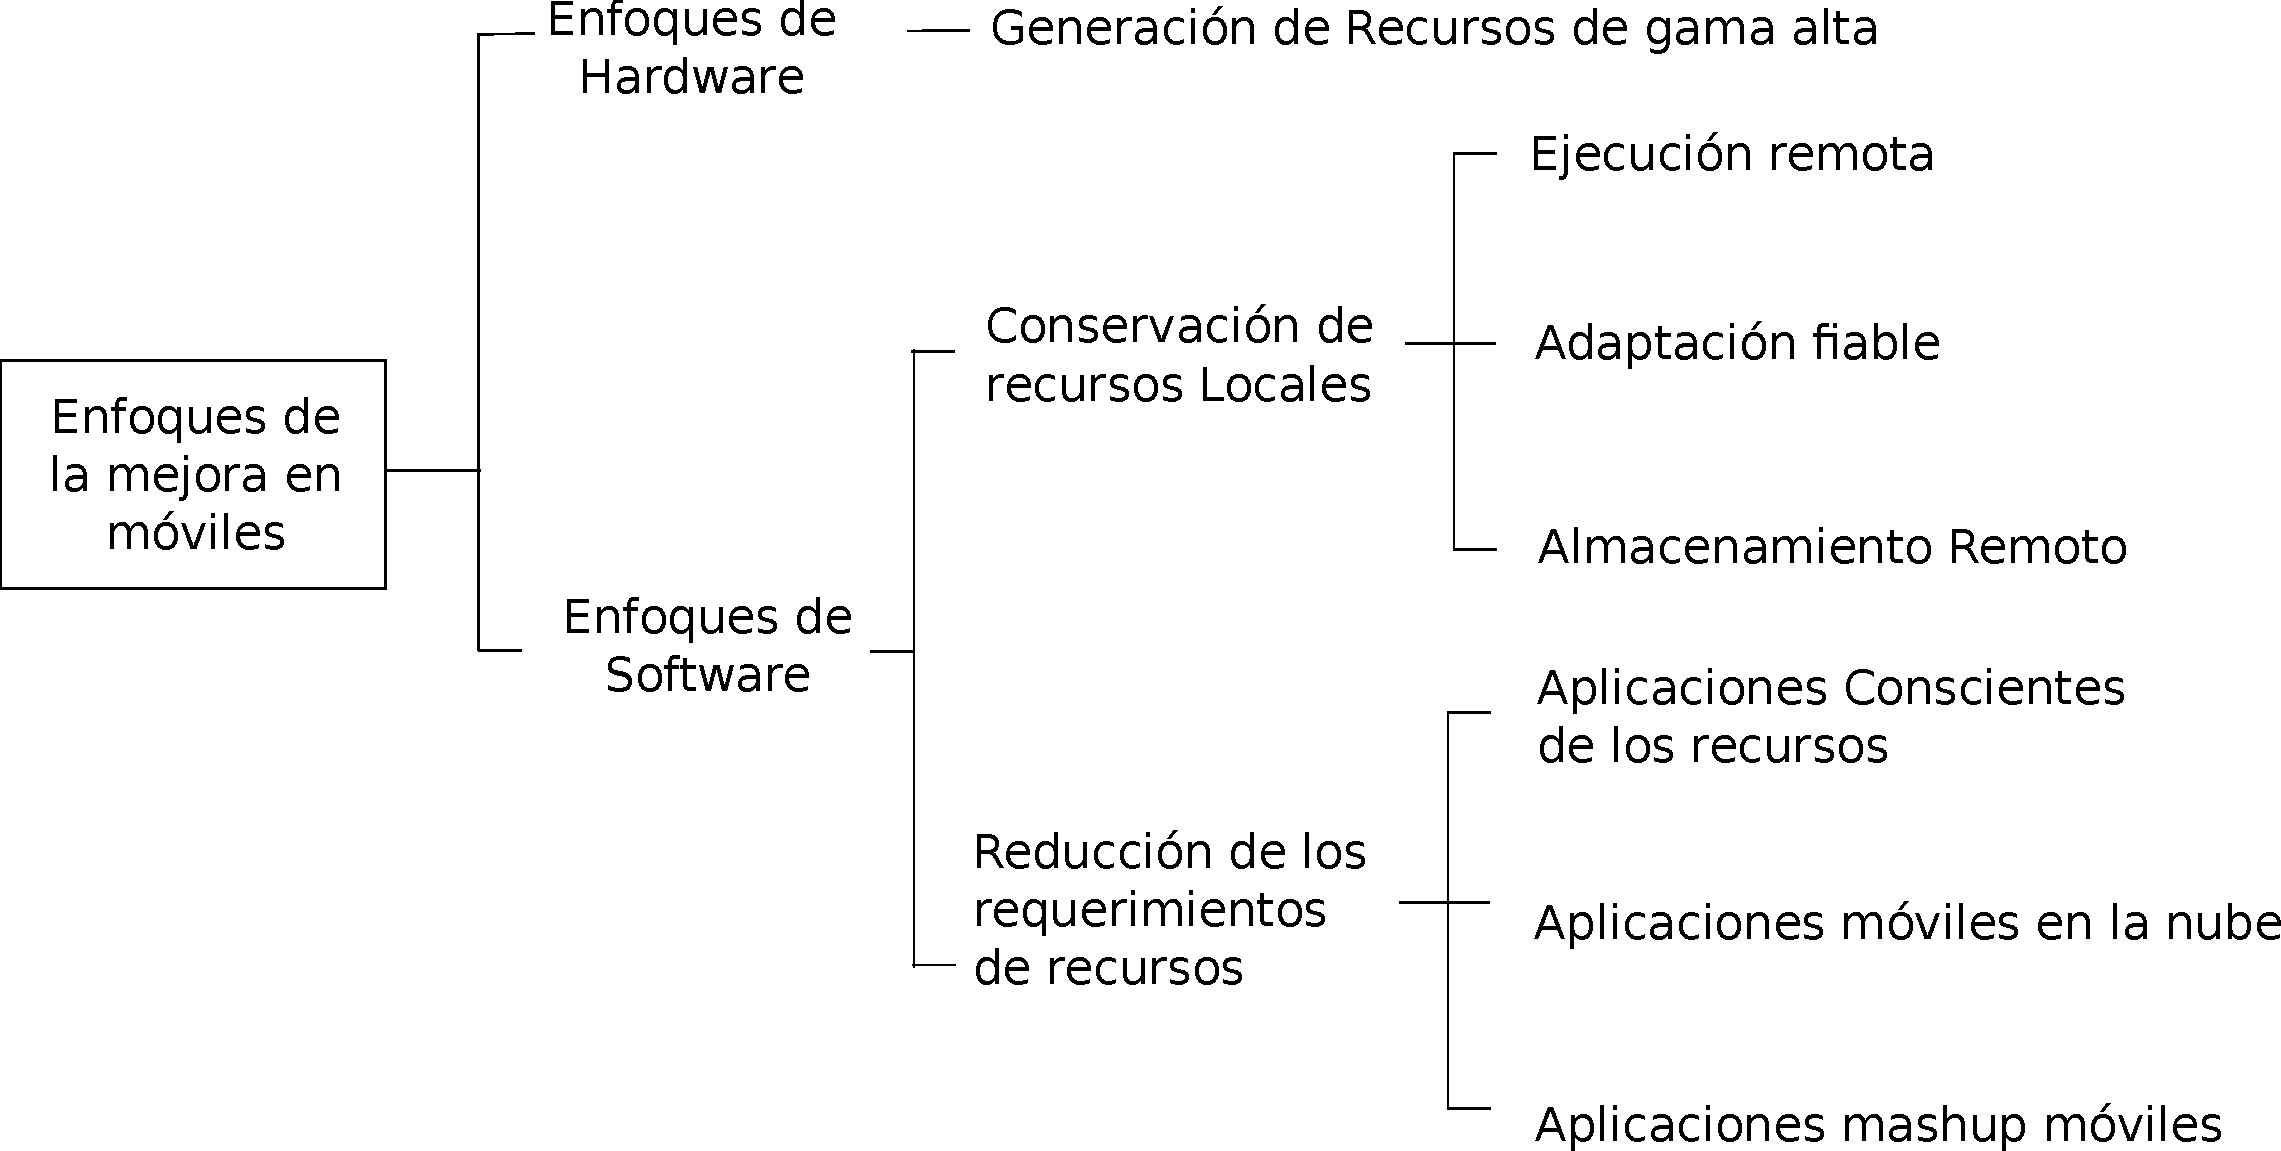
\includegraphics[scale=0.35]{Figures/taxonomySmartphone.pdf}
 \caption{Taxonomía de los enfoques de mejora de en móviles. Figura adaptada de \cite{abolfazli2012mobile}}
 \label{fig:approachesmobileaugmentation}
\end{figure}

\section{Heterogeneidad}

La innegable popularidad que han tomado los dispositivos móviles como los smartphones, wereables y objetos de IoT crea un mercado dinámico
y exigente, que ha diversificado a los componentes de MCC en diferentes dimensiones de una manera no estándar. Esta variedad de hardware, arquitecturas,
infraestructura y tecnologías de dispositivos móviles, nubes, y redes inalámbricas genera un entorno Heterogéneo. En esta sección
describimos como la heterogeneidad abarca a todos los componentes de MCC: computación móvil, computación en nube y redes inalámbricas
\cite{sanaei2014heterogeneity}. Este
escenario es representado en la Figura \ref{fig:mccheterogeinity}. Aunque la heterogeneidad en la MCC ha sido inherente desde los orígenes
de la computación en nube y móvil, su complejidad la hace desafiante y única, por lo que necesita un estudio exhaustivo.


\subsection{Taxonomía en la MCC}

En este apartado estudiaremos detalladamente la heterogeneidad en MCC por medio del análisis de sus orígenes y dimensiones. 
Según \cite{sanaei2014heterogeneity}, 
los orígenes de la heterogeneidad se dan por el hardware, plataforma, característica, API, red y dispositivos. 


\begin{figure}[h]
 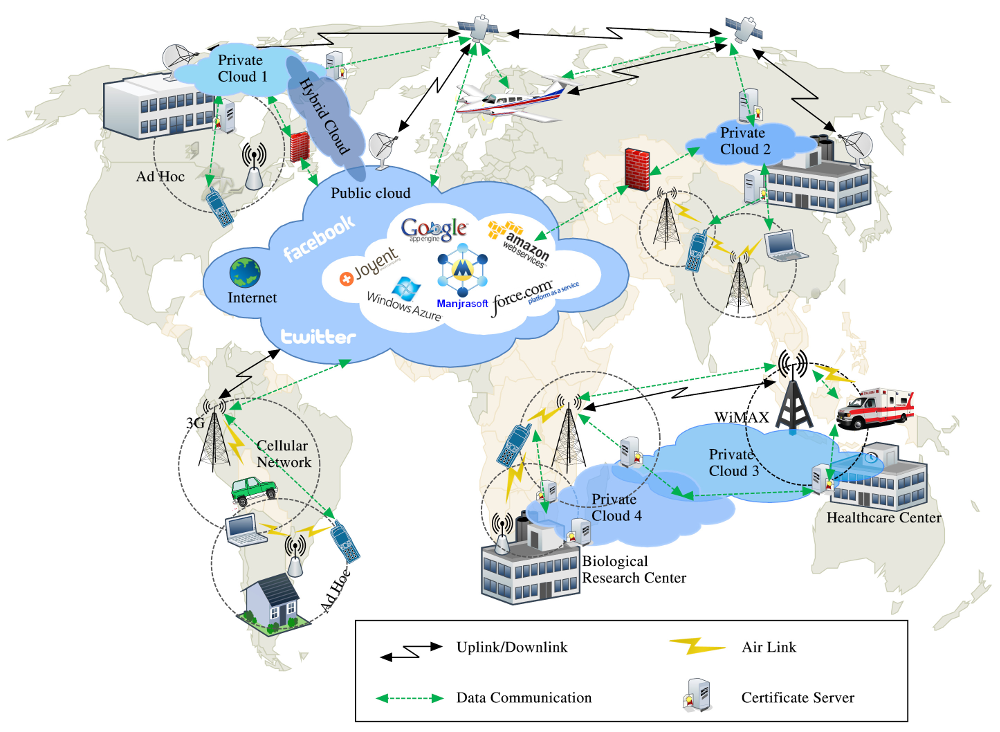
\includegraphics[scale=0.45]{Figures/mccheterogeinity}
 \caption{Una vista general a MCC \cite{sanaei2014heterogeneity}}
 \label{fig:mccheterogeinity}
\end{figure}

\subsubsection{Orígenes de la heterogeneidad en MCC}

Para entender claramente la heterogeneidad que no es una característica específica de un dominio, podemos percibir casos en la vida real:
los automóviles que están compuestos de partes totalmente diferentes que logran interactuar entre ellos con un solo fin; el caso de las
partes del cuerpo que
son intrínsecamente heterogéneas logran cooperan para mantener la funcionalidad como un todo. Análogamente, los tres componentes principales 
de la MCC (computación en la nube, computación móvil y redes inalámbricas) deben interactuar sin problemas y consistentemente. Esta división 
de los orígenes de la taxonomía está representada en la imagen de la Figura \ref{fig:heterogeinityRootsmcc}. 


\begin{figure}[h]
 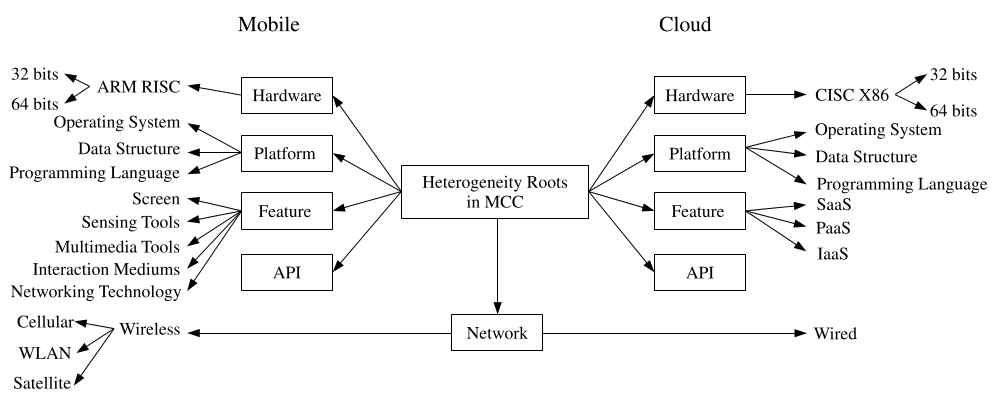
\includegraphics[scale=0.45]{Figures/heterogeinityRootsmcc}
 \caption{Taxonomía de los orígenes de la heterogeneidad en MCC \cite{sanaei2014heterogeneity}}
 \label{fig:heterogeinityRootsmcc}
\end{figure}


\begin{enumerate}
 \item \textbf{Heterogeneidad de hardware:} La fuerte demanda de los usuarios de móviles y la competencia entre las grandes compañías 
 fabricantes de hardware han permitido que diversifiquen sus arquitecturas internas entre dispositivos móviles, servidores en nube, e 
 infraestructuras de redes. 
 
 En el entorno de la computación en nube, la variedad de proveedores de servidores otorgan una variedad en infraestructuras y diseño 
 de arquitecturas de Computadoras con un Conjunto de Instrucciones Complejas (CISC, por sus siglas en inglés) con las variaciones de 32 y
 64 bits. 
 
 Similarmente, la diversidad de arquitecturas en los dispositivos móviles, que generalmente están basadas en Computadoras con Conjunto de Instrucciones
 Reducidas (RISC, por sus siglas en inglés) de 32 bits; sin embargo, existe una considerable variación en términos de velocidad del procesador,
 número de nucleos, cantidad de caché del procesador. Igualmente existe una variedad importante entre los recursos del dispositivo móvil como
 la memoria memoria interna, fiabilidad de la antena inalámbrica y la capacidad de la batería.
 
 La heterogeneidad en hardware entre los dispositivos móviles y las computación en nube, crea los siguientes problemas: 
 
 \begin{itemize}
  \item La variación de hardware de los servidores en nube conlleva a una diferencia de rendimiento y calidad de servicio, además  del casi nulo
  soporte para la portabilidad de aplicaciones entre los diferentes proveedores, entonces fuerza al usuario a tomar una decisión 
  importante entre la vasta cantidad de opciones disponibles. Los desarrolladores pueden usar la herramienta en línea de \textit{Software Insider}
  para optar por la mejor propuesta de servicios en nube \footnote{\url{http://cloud-computing.softwareinsider.com}, último acceso en setiembre 2015}.
  \item El conocido principio usado por desarrolladores ``codifica una vez, ejecútalo donde sea'' se cumple parcialmente en el 
  heterogéneo ambiente móvil, dado que requiere dependencia de herramientas privadas  
  multi-plataforma como Xamarin \footnote{ \url{http://xamarin.com/}, último acceso en setiembre 2015} o Qt para móviles 
  \footnote{ \url{http://www.qt.io/mobile-app-development/}, último acceso en setiembre 2015}
  . Las herramientas en mención son un gran aporte en el entorno de los \textit{smartphones} pero tienen
  una limitante en entornos de dispositivos \textit{weareables} y de Internet de las cosas, ya que en su arquitectura se ejecuta sobre diferentes
  distribuciones ligeras de Linux.
  \item Un parámetro fundamental en las técnicas de \textit{offloading} es la estimación precisa de la energía \cite{sanaei2014heterogeneity},
  para
  que se decida si el enviar partes de la aplicación conservará energía o no \cite{5445167}. Es por tal motivo que se necesita estimar de manera precisa
  este valor 
  
 \end{itemize}

 \item \textbf{Heterogeneidad de Plataforma:} De modo equivalente a la heterogeneidad de hardware, existe una amplia disponibilidad de sistemas
 operativos, lenguajes de programación y estructuras de datos en MCC que transforman a las plataformas en entornos heterogéneos. En el contexto
 de los sistemas operativos móviles encontramos algunos como Android \footnote{\url{http://developer.android.com/index.html}, último acceso en setiembre 2015} y iOS 
 \footnote{\url{https://developer.apple.com/devcenter/ios/index.action}, último acceso en setiembre 2015}, de Google y Apple respectivamente,
 cada uno con múltiples versiones
 y  arquitecturas que soportan diferentes lenguajes de programación y estructuras de datos. Android ofrece el desarrollo sobre la máquina virtual 
 de java basado en bytecodes; mientras que iOS soporta Objective-C, un lenguaje compilado a nivel de código máquina.
 
 En en ámbito de la computación en nube los proveedores más populares tales como App Engine
 \footnote{\url{https://cloud.google.com/appengine/docs}, último acceso en setiembre 2015}, Microsoft Azure
 \footnote{\url{https://azure.microsoft.com/en-us/}, último acceso en setiembre 2015} y 
 Amazon Web Services \footnote{\url{http://aws.amazon.com/}, último acceso en setiembre 2015} soportan una diversa cantidad de lenguajes de programación, sistemas operativos
 y arquitecturas de almacenamiento, p. ej. Azure Soporta .Net, PHP, Ruby, Python y Java para desarrollar aplicaciones, Google 
 igualmente ofrece Java además de Python, PHP y Go; sin embargo, estas plataformas poseen almacenes de datos no relacionales con diseños 
 estructurales y esquemas de particionado diferentes (Big table de Google \cite{Chang:2006:BDS:1267308.1267323}, Dynamo de Amazon \cite{decandia2007dynamo} y 
 DocumentDB de Azure 
 \footnote{\url{http://azure.microsoft.com/en-us/services/documentdb/}, último acceso en setiembre 2015}), y por lo tanto estos proveedores hacen cumplir  sus restricciones
 de uso  para proveer mayor flexibilidad de su servicio.
 
 Tal heterogeneidad convierte la portabilidad en un proceso tedioso, costoso y de alto riesgo. Transferir aplicaciones entre diferentes
 nubes demanda un costo extra que incluye descargar la aplicación, realizar la conversión y desplegar el nuevo sistema a la nueva nube. Es
 peligroso, dado que la transferencia entre bases de datos de entre nubes compromete la privacidad e integridad de los datos cuando existe una
 diferencia entre sistemas de archivos y técnicas de encriptación \cite{5708456}. Por lo tanto, para el desarrollador escoger la plataforma 
 correcta no es tarea fácil. La variedad de plataformas se representa en la Figura \ref{fig:difficultDecisiton}.
 
 \begin{figure}[h]
 \centering 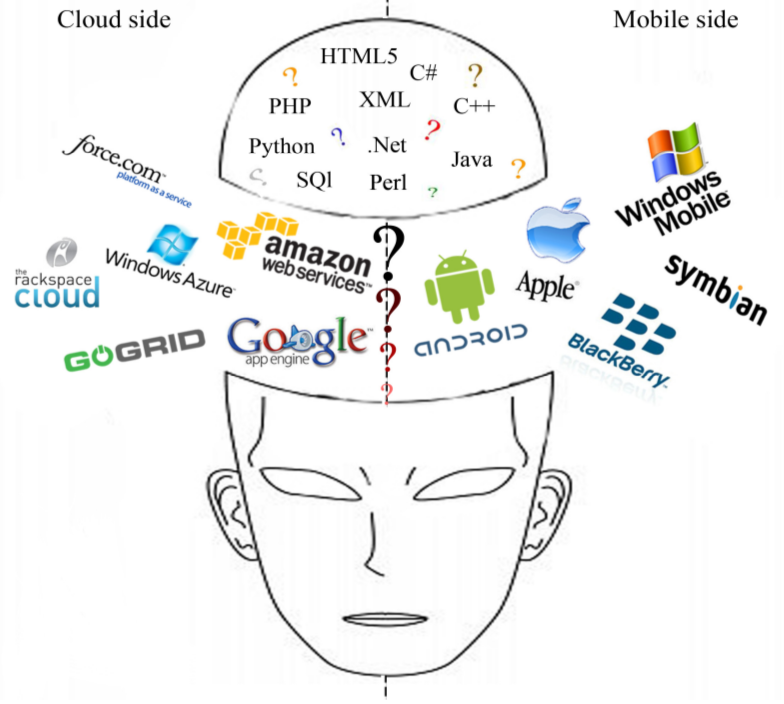
\includegraphics[scale=0.3]{Figures/difficultDecisiton}
 \caption{Heterogeneidad de plataformas en MCC y la difícil tarea para el desarrollador elegir la correcta \cite{sanaei2014heterogeneity}}
 \label{fig:difficultDecisiton}
\end{figure}
 
 %falta un poco hablar de las soluciones como phonegap o marmalade
 
 % La portabilidad como la define el Comité Internacional para los Estándares de Tecnologías de la Información (INCITS, por sus siglas en inglés) 

 
 \item \textbf{Heterogeneidad de Características: } Es la variación de características en los \textit{smartphones} tales como los sensores,
 el área de visualización,  multimedia, y tecnologías de red. Una de las características que más varía entre fabricantes es la cámara. P. ej.
 El celular motorola X, un celular de gama media, posee una cámara de 10PM \footnote{\url{https://www.motorola.com/us/Moto-X/FLEXR1.html}, 
 último acceso en setiembre 2015}, entretanto 
 el celular Samsung Galaxy Edge 6, un celular de gama alta, dispone de una cámara de 16 MP \footnote{\url{http://www.samsung.com/uk/galaxys6/}, 
 último acceso en setiembre 2015}. Esta
 desigualdad puede significar una variación en las técnicas de offloading ( las cuales detallaremos en el Capítulo \ref{ch:Chapter4}) 
 si es que consideramos algún tipo de procesamiento de imagen en la nube,  debido a que el envío de datos a la nube sería más lento.
 
 Las variaciones en el área de visualización entre los celulares impiden que los desarrolladores diseñar una interfaz de usuario que se adapte a 
 todos los tamaños de pantalla, disminuyendo la experiencia de usuario.	En el entorno Android existe el soporte para la construcción de 
 aplicaciones que se adecúan al contenido de la pantalla en su versión 3.2 en adelante \footnote{
 \url{http://developer.android.com/about/versions/android-3.2.html}, último acceso en setiembre 2015}.
 
 La heterogeneidad en nube está dada por los servicios que cada proveedor ofrece en particular. P. ej. \textit{Google App Engine} ofrece el servicio 
 de Big Query \footnote{\url{https://cloud.google.com/bigquery/}, último acceso en setiembre 2015} que permite a los administradores
 realizar consultas sobre \textit{Big Data} 
 en tiempo real. Microsoft Azure a su vez, es el único que ofrece un servicio de almacenamiento de backups encriptado 
 \footnote{\url{http://azure.microsoft.com/en-us/services/backup/}, último acceso en setiembre 2015} 
  
  \item \textbf{Heterogeneidad de APIs:} Las Interfaces de Programación de Aplicaciones (API, por sus siglas en inglés) son bibliotecas de código
  que permiten un acceso rápido a datos específicos o funciones de un proveedor en particular. Los usuarios de \textit{smartphones} tienen una 
  alta expectativa respecto a la experiencia de usuario, es por tal motivo que las mas grandes compañías de sistemas operativos móviles (Android, iOS, 
  Blackberry \footnote{\url{http://us.blackberry.com/}, último acceso en setiembre 2015} y Firefox OS 
  \footnote{\url{https://www.mozilla.org/en-US/firefox/os/2.0/}, último acceso en setiembre 2015}) otorgan una amplia
  gama de APIs a los desarrolladores. Esta es una ventaja para desarrollar aplicaciones enriquecedoras en experiencia de usuario, de una forma 
  ágil y fácil sin necesidad de acceder al kernel. Sin embargo, las APIs son dependientes de los proveedores y la portabilidad nuevamente se
  convierte en una tarea complicada, dadas las diferencias de las APIs.
  
  De manera similar, en la computación en nube, la casi totalidad de proveedores diseñan APIs que son usados exclusivamente por sus clientes
  p. ej. Google App engine ofrece la API de documentos e Indices \footnote{\url{https://cloud.google.com/appengine/docs/java/search/}, último acceso en setiembre 2015} 
  para realizar búsquedas de manera rápida y eficiente sobre espacios geográficos y texto principalmente. Otro ejemplo que resaltamos es 
  en el envío de notificaciones push, Google, Azure y Parse \footnote{\url{https://www.parse.com/}, último acceso en setiembre 2015}
  ofrecen sus APIs basadas en 
  \textit{Google Cloud Messaging} \footnote{\url{https://developer.android.com/google/gcm/index.html}, último acceso en setiembre 2015}
  , \textit{Notification Hubs} 
  \footnote{\url{http://azure.microsoft.com/en-us/documentation/services/notification-hubs/}, último acceso en agosto 2015} y \textit{Parse Push Notifications} 
  \footnote{\url{https://parse.com/docs/push_guide}, último acceso en julio 2015} respectivamente. Esta heterogeneidad además que impide la portabilidad, 
  demanda un tiempo considerable al desarrollador poder aprender cada una de las APIs en nube.
  
  \item \textbf{Heterogeneidad de Redes:} A diferencia de las computadoras de escritorio, la mayoría de dispositivos móviles solamente usan redes
  inalámbricas para conectarse a Internet, las cuales son comparativamente más intermitentes y menos fiables. La variedad infraestructuras
  de redes inalámbricas disponibles como Wi-fi, 3G y 4G dificultan el proceso de selección de la red más adecuada en el momento que el cliente
  móvil está en movimiento.
  
  
  
 
 
\end{enumerate}

